% !TEX root = ../thesis.tex

\documentclass[thesis.tex]{subfiles}


\begin{document}

\chapter{Introduction}
\label{chapter:intro}

aiheen rajaus johdantoon
% http://ipimediaworld.com/wp-content/uploads/2013/10/Turning-your-smartphone.pdf

Johdanto selvittaa samat asiat kuin tiivistelma, mutta laveammin. Johdannossa kerrotaan yleensa seuraavat asiat

Kuten kirjallisessa osassa todettiin, vaarentajat pyrkivat selvittamaan tekniikan periaatteen nopeasti, joten turvallisuussovelluksissa kaytettavia merkintoja on oltava riittavan monimutkaisia ja niita on voitava muunnella helposti. Kuten luvuissa 2.1.1-2.1.2 todettiin, luminoforien luminesenssiominaisuudet muuttuvat yhdisteen rakenteen muuttuessa. Erilaisten rakenteiden suunnitelmallinen synteesi onkin tarkeaa, mikali tekniikkaa halutaan kehittaa eteenpain. Luminoforien viritys- ja emissioaallonpituuksien tulisi soveltua myos kaytetyn laitteiston vaatimuksiin.

\begin{itemize}
\item[--]Tutkimuksen taustaa ja tutkimusaiheen yleisluonteinen esittely
\item[--]Tutkimuksen tavoitteet
\item[--]Paakysymys ja osaongelmat
\item[--]Tutkimuksen rajaus ja keskeiset kasitteet.
\end{itemize}

Product authentication, or brand protection, ...

aiheen rajaus johdantoon
fotoluminesenssiin perustuva pintamerkkiaineteknologia
This thesis explores an alternative, competing technology.

The focus of this thesis is the design and implementation of a scalable hybrid mobile application. The application will be developed as a part of the LuminoTrace project at Aalto CHEM for the purposes material verification. The functionality of the application can be briefly described as follows:

\begin{enumerate}
\item A user takes an image of a material with his/her mobile device
\item An algorithm analyzes the image and returns a unique digital fingerprint
\item The fingerprint is compared against a database of fingerprints
\item The user is notified whether or not a match was found.
\end{enumerate}

The verification is done by analyzing the spectrum of a special chemical compound embedded in the material. Both the underlying algorithm and the compound have already been developed as a part of the LuminoTrace project.

The implementation of the application can be divided into the following tasks:

\begin{itemize}
\item[--]Access and control built-in camera of the mobile device
\item[--]Port the code of the spectrum analysis algorithm to JavaScript
\item[--]Implement the UI
\item[--]Implement the back end infrastructure (cloud)
\end{itemize}

\begin{figure}[hb]
\centering 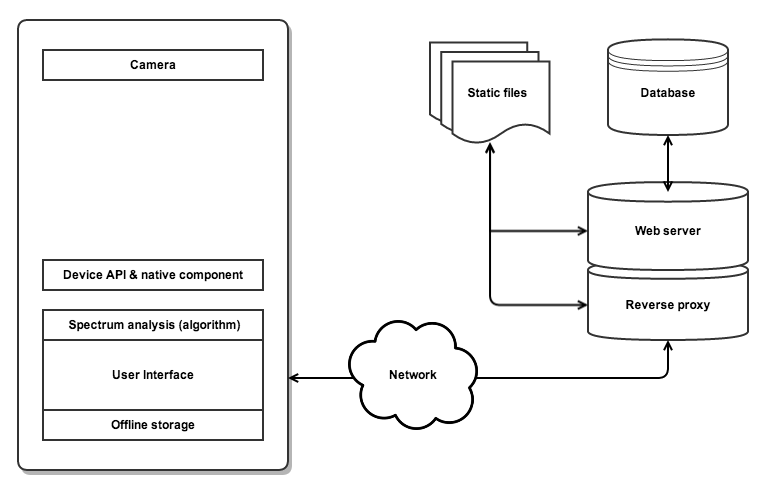
\includegraphics[width=13.25cm]{images/diagram_0404}
\caption{A high-level overview of the structure of the application \label{fig:diagram}}
\end{figure}

The functionality outlined above can be largely achieved by utilizing existing Web technologies and the W3C Device APIs. However, a more granular control over the camera (e.g. burst-mode, flash settings) will require a native component to be implemented for each target platform. The preliminary target platform will be Windows Phone (WP). To improve scalability the fingerprint will be computed on the client-side. This will require for the existing algorithm to be ported into JavaScript. Scalability can be further improved by offloading parts of the (fingerprint) database from the server to the user's device. Moreover, usability is improved as the application can function offline without the overhead of network latency. Hosting fingerprint data on the user's device might however have security implications: can the data be safely/efficiently encrypted on the user's device?

A high-level overview of the main components and interfaces of the application described above is given in Figure \ref{fig:diagram}.

\section{Research Questions}

TBD

\begin{itemize}
	\item \textbf{RQ1}: What factors need to be considered when analyzing photoluminescent material using a smartphone?
	- usability (time constraints)
	- luminophors
	- differences between cameras/vendor APIs
	\item \textbf{RQ2}: What are the reasons for and against storing data client-side?
	- offline func. (sync \& its implementation costs)
	- security
\end{itemize}


\end{document}